\documentclass[10pt, a4paper, twoside]{article}

% Set up the standard margins for the document
% 42.2 left & 15.5 right is same as Forsling, Neymark
% 21.3 top  & 20 bottom is same as Olofsson
\usepackage[left=19.5mm, right=19.5mm, top=21.3mm, bottom=20mm]{geometry}

\usepackage{subcaption}
\usepackage{float}

% Input file character encoding (kinda useless if we don't
% use åäö and stuff, but it doesn't hurt to have it)
\usepackage[utf8]{inputenc}
%\usepackage[swedish]{babel}

% Block Comments
\usepackage{comment}

% No indentation in new paragraph
\usepackage{parskip}

% To include graphics
\usepackage{graphicx}

% More mathematical symbols and fonts
\usepackage{amsmath}
\usepackage{amsfonts}
\usepackage{amssymb}

% Simple list
\usepackage[ampersand]{easylist}
\ListProperties(Hide=100, Hang=true, Progressive=5ex, Style*=$\bullet$ ,
Style2*=-- ,Style3*=$\circ$ ,Style4*=\tiny$\blacksquare$ )


% Clickable internal links
\usepackage{hyperref}
\usepackage[all]{hypcap} % without this the link takes you to the caption, not the top of the image
\hypersetup{ % Settings for links in documnet
	setpagesize = false, % Don't allow hyperref to change page size. Tips från Micke Olofsson
	colorlinks = true,   % No boxes around links
	linkcolor = black,citecolor = black,filecolor = black,urlcolor = black, % don't color links
}

% To include to first page pdf file
\usepackage{pdfpages}

% Add section number to equation and figure number (ex: 5.11 instead of simply 11)
\numberwithin{equation}{subsection}
\numberwithin{figure}{section}
\numberwithin{table}{section}

% Show program code listings in document
\usepackage{listings}

%
% Header stuff
%
\usepackage{fancyhdr}
\setlength{\headheight}{15pt}

\fancyhf{}
\fancyhead[LE, RO]{\thepage}
\fancyhead[RE]{TSBK03 2013: Technical Report}
\fancyhead[LO]{Extrapolate and Conquer}

\fancypagestyle{plain}{ %
\fancyhf{} % remove everything
\renewcommand{\headrulewidth}{0pt} % remove lines as well
\renewcommand{\footrulewidth}{0pt}}
%
% End header stuff
%




\begin{document}

% First page
\includepdf{Cover/cover.pdf}


% Project identity page
\newpage
\pagestyle{fancy}
\pagenumbering{roman}
\setcounter{page}{2} % sets the current page number to 2 

\begin{center}
    \vspace*{4\baselineskip}

	\textbf{\huge Extrapolate and Conquer} \\
	\vspace*{0.5\baselineskip}
	Teknik för avancerade datorspel, HT 2013 \\
	Department of Electrical Engineering (ISY), Linköping University
	
	\vspace*{2\baselineskip}
	\textbf{\LARGE Participants}


	{\footnotesize 
	\begin{tabular}{|p{2.7cm}|p{1cm}|p{2cm}|p{3.4cm}|}
		\hline
		\textbf{Name} & \textbf{Tag} & \textbf{Phone} & \textbf{E-mail} \\
		\hline
		Gustav Häger & GH & 070--649\,03\,97 & gusha124@student.liu.se \\
		\hline
		Alexander Sjöholm & AS & 076--225\,11\,74 & alesj050@student.liu.se \\
		\hline
		Mattias Tiger & MT & 073--695\,71\,53 & matti166@student.liu.se \\
		\hline
	\end{tabular}
	}

{\footnotesize 
\vspace{0.5\baselineskip}
\vspace{1\baselineskip}

\textbf{Examiner}: Ingemar Ragnemalm, ingis@isy.liu.se \\
}

\end{center}



% table of contents
\newpage
\tableofcontents
\listoffigures
\listoftables

% Blank page
%\newpage
%\thispagestyle{empty}
%\mbox{}



%
% Content start
%
\newpage
\pagenumbering{arabic}

\newpage
\section{Introduction}
\label{sec:introduction}
The aim of this project was to develop a computer graphics application combining several state-of-the-art techniques into one beautiful and intelligent world. 


\newpage
\section{System Core}
\label{sec:Core}
Complex entity system..

\subsection{Rendering}

\subsection{Physics}



\newpage
\section{Graphics}
\label{sec:Graphics}
\section{Generating a World}

A world is easily divided into different aspects. There are the sky, the oceans and the land. The land contain different terrain, with different types of ground and vegetation. There is a sun orbiting the world, casting rays of light and in the process creating reflections and indirectly making shadows.\\
\\
A procedural world is generated by carefully chosen algorithms. Our world is procedurally generated anew in a new unique constellation on every run, or a seed can be provided to generate specific worlds. The terrain is first formed, then the ground texturing and the vegetation, both dependent on properties of the terrain. The shadows depend on the sun and the waves on the terrain as well as on time itself.

\subsection{Sky}
The sky is achieved using a high-resolution texture of a sky mapped to a skybox. The mathematical location of the sun is placed as close as possible to the sun appearing in this texture. This gives shadows and shading a natural feel. The texture has been manually modified at the horizon to fade towards a shadowish gray color. The color is the same as the one objects are distance-fogged with. This makes the sky melt into the ocean in a very nice way. 

\subsection{Ocean}
The water is made up of a normal-mapped square and a blue color. The normal map is repeated over the square and is moving in texture space, giving the illusion of a wind. The normal map movement cycles such that when the water normal map has been totally displaced, it starts over again from its original position. This movement makes the water glitter from a far, see figure \ref{fig:water}.
\begin{figure}[H]
\begin{subfigure}{.5\textwidth}
  \centering
  \includegraphics[width=0.9\linewidth]{images/waterWaves.jpg}
  \caption{The water.}
  \label{fig:waterWaves}
\end{subfigure}%
\begin{subfigure}{.5\textwidth}
  \centering
  \includegraphics[width=0.9\linewidth]{images/waterGlimmer.jpg}
  \caption{Glittering water.}
  \label{fig:waterGlistering}
\end{subfigure}
\caption[Noise comparison]{\textit{Comparison of noise functions}}
\label{fig:water}
\end{figure}
Waves on the beaches is made by having several sinus waves aggregate horizontally to vary the wave fronts, and by having a sinus wave that control the vertical assent/decent of the waves. It is hard to catch on a screen shot, but an image of the waves in the world is shown in figure \ref{fig:waves}
\begin{figure}[H]
  \centering
  \includegraphics[width=0.9\linewidth]{images/waves.jpg}
  \caption{The waves are seen at the beach.}
  \label{fig:waves}
\end{figure}%
The sky is reflected in the water by using an image which is the projection of the sky onto the ocean as a texture for the water. This texture is moving with the camera in the xz-plane. An example is seen in figure \ref{fig:skyReflection}. It could be improved in the future by taking the height of the camera in consideration as well, or to continuously project the sky onto the water according to the camera position. Currently the camera height do not change the reflection, making it a bit unrealistic if moving up and down.
\begin{figure}[H]
  \centering
  \includegraphics[width=0.9\linewidth]{images/reflectingSky.jpg}
  \caption{The sky reflected in the ocean.}
  \label{fig:skyReflection}
\end{figure}%

\newpage
\subsection{Terrain}
The terrain is generated by sampling a noise function and transforming its value into a height for each vertex. The noise in this case originates from a Simplex function. However, to get a realistically looking terrain it is not sufficient to sample this function only once for every vertex.

Fractional Brownian Motion is calculated by sampling the Simplex function at different frequencies and calculating a weighted sum over the samples \cite{FracBrownMotion}. The result is a nice looking height map. This allows for an arbitrary sample density, see figure \ref{fig:textureDensityComparison1} which show a few different sample densities. A further possible extension would be to use tessellation, which would allow for a terrain with arbitrary fine details.  

\begin{figure}[H]
\begin{subfigure}{.5\textwidth}
  \centering
  \includegraphics[width=0.9\linewidth]{images/Simplex.jpg}
  \caption{Height map generated from single-octave simplex noise}
  \label{fig:sub1}
\end{subfigure}%
\begin{subfigure}{.5\textwidth}
  \centering
  \includegraphics[width=0.9\linewidth]{images/FracBrownMotion.jpg}
  \caption{Height map generated with Fractional Brownian Motion}
  \label{fig:sub2}
\end{subfigure}
\caption[Noise comparison]{\textit{Comparison of noise functions}}
\label{fig:R_kitchen_example}
\end{figure}

The height map is finally assured to always slope into the ocean. This is done by first setting the all edge values to zero, then weighting the entire map with a thresholded Gaussian kernel, see figure \ref{fig:heightMapConstruction} below. 

\begin{figure}[H]
\begin{subfigure}{\textwidth/3}
  \centering
  \includegraphics[width=0.9\linewidth]{images/heightMapRaw.jpg}
  \caption{Height map with edge set to zero.}
  \label{fig:heightMapRaw}
\end{subfigure}%
\begin{subfigure}{\textwidth/3}
  \centering
  \includegraphics[width=0.9\linewidth]{images/heightMapKernel.jpg}
  \caption{Thresholded Gaussian kernel}
  \label{fig:heightMapKernel}
\end{subfigure}
\begin{subfigure}{\textwidth/3}
  \centering
  \includegraphics[width=0.9\linewidth]{images/heightMapFinal.jpg}
  \caption{Final height map.}
  \label{fig:heightMapFinal}
\end{subfigure}
\caption[Height map construction]{\textit{All steps in the creation of the height map.}}
\label{fig:heightMapConstruction}
\end{figure}

\begin{figure}[H]
\begin{subfigure}{.5\textwidth}
  \centering
  \includegraphics[width=0.9\linewidth]{images/terrainDensityComparison1_05.jpg}
  \caption{Density 0.5}
  \label{fig:textureDensity05}
\end{subfigure}%
\begin{subfigure}{.5\textwidth}
  \centering
  \includegraphics[width=0.9\linewidth]{images/terrainDensityComparison1_1.jpg}
  \caption{Density 1.0}
  \label{fig:textureDensity1}
\end{subfigure}%

\begin{subfigure}{.5\textwidth}
  \centering
  \includegraphics[width=0.9\linewidth]{images/terrainDensityComparison1_2.jpg}
  \caption{Density 2.0}
  \label{fig:textureDensity2}
\end{subfigure}%
\begin{subfigure}{.5\textwidth}
  \centering
  \includegraphics[width=0.9\linewidth]{images/terrainDensityComparison1_5.jpg}
  \caption{Density 5.0}
  \label{fig:textureDensity5}
\end{subfigure}%

\begin{subfigure}{.5\textwidth}
  \centering
  \includegraphics[width=0.9\linewidth]{images/terrainDensityComparison1_10.jpg}
  \caption{Density 10.0}
  \label{fig:textureDensity10}
\end{subfigure}%
\begin{subfigure}{.5\textwidth}
  \centering
  \includegraphics[width=0.9\linewidth]{images/terrainDensityComparison1_15.jpg}
  \caption{Density 15.0}
  \label{fig:textureDensity15}
\end{subfigure}%
  \caption{A comparison of different vertex and sample density, from 0.5 to 15 vertexes per OpenGL length units. Waves are shown in some of the images, as the wave generator currently doesn't distinguish between lakes and oceans.}
  \label{fig:textureDensityComparison1}
\end{figure}

\newpage
\subsection{Ground}
The ground is textured using a non-linear multi-texturing approach based on both altitude and terrain slope. Currently only three textures are used: one sandy, one grassy and one rocky, which can be seen in figure \ref{fig:textures}. These textures were generated in Spiral Graphics Genetica Viewer and are procedurally generated tiling textures.

\begin{figure}[H]
\begin{subfigure}{\textwidth/3}
  \centering
  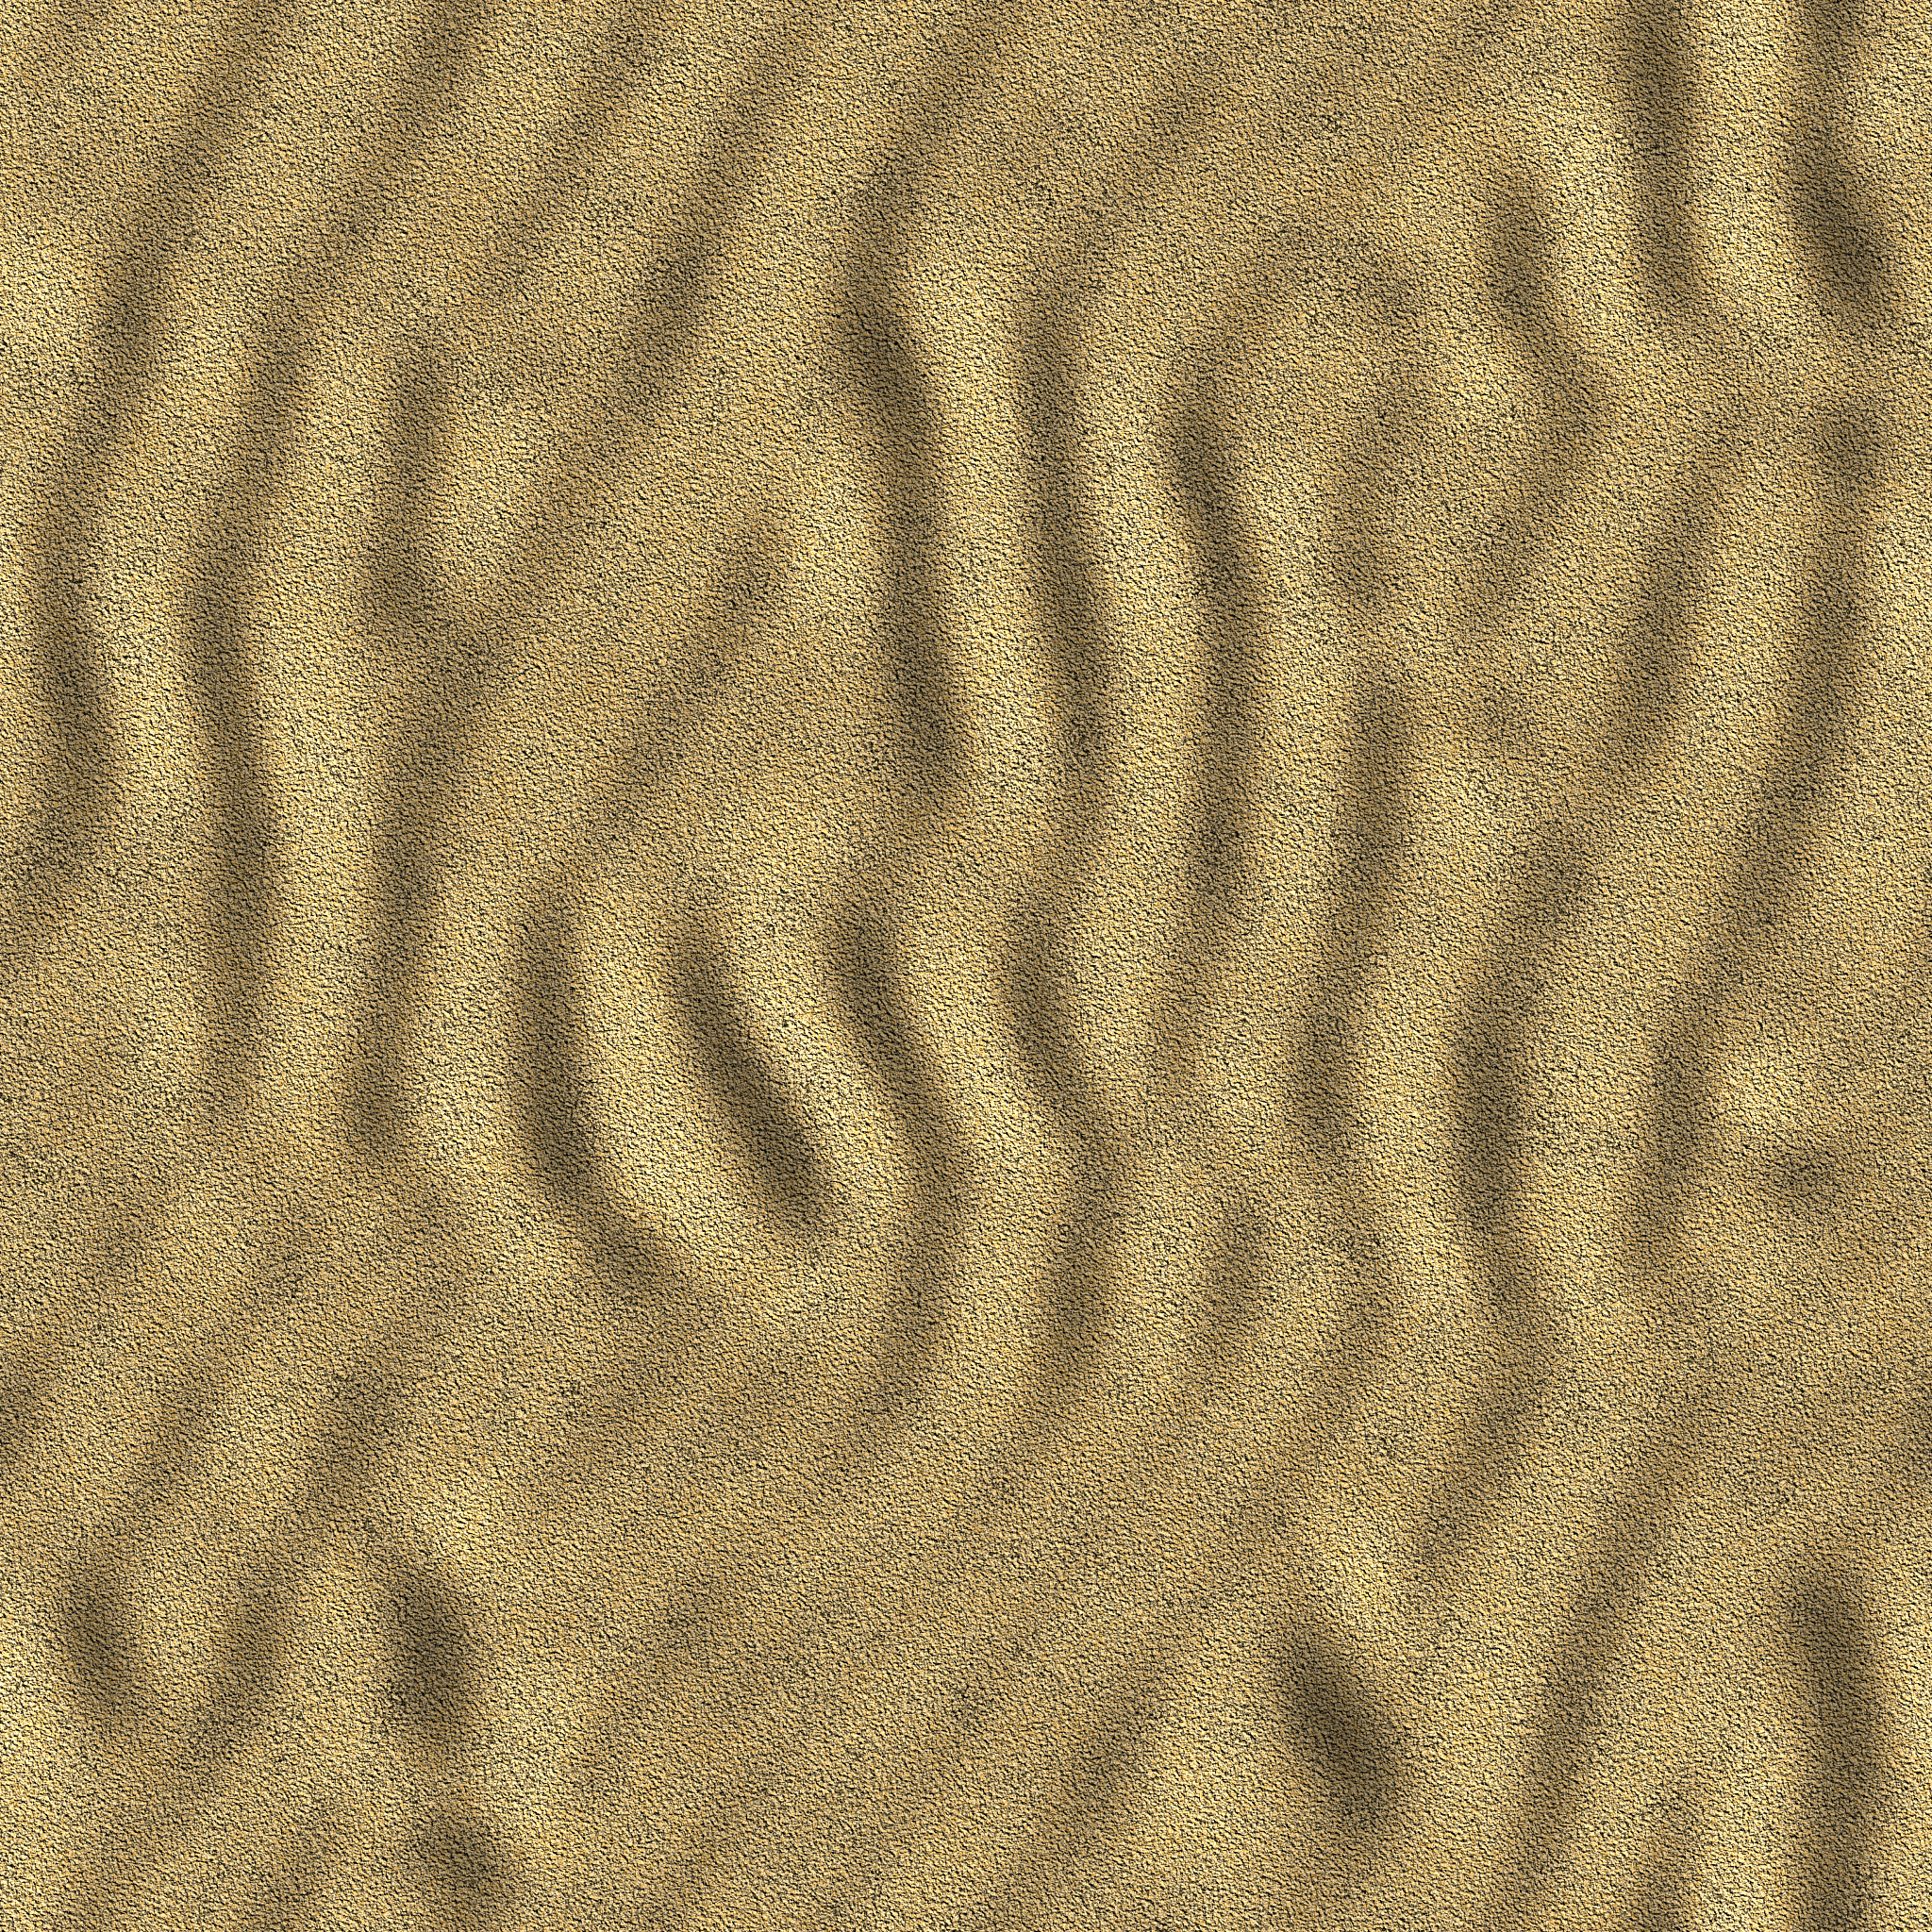
\includegraphics[width=0.9\linewidth]{images/textureSand.jpg}
  \caption{The sand/beach texture.}
  \label{fig:textureSand}
\end{subfigure}%
\begin{subfigure}{\textwidth/3}
  \centering
  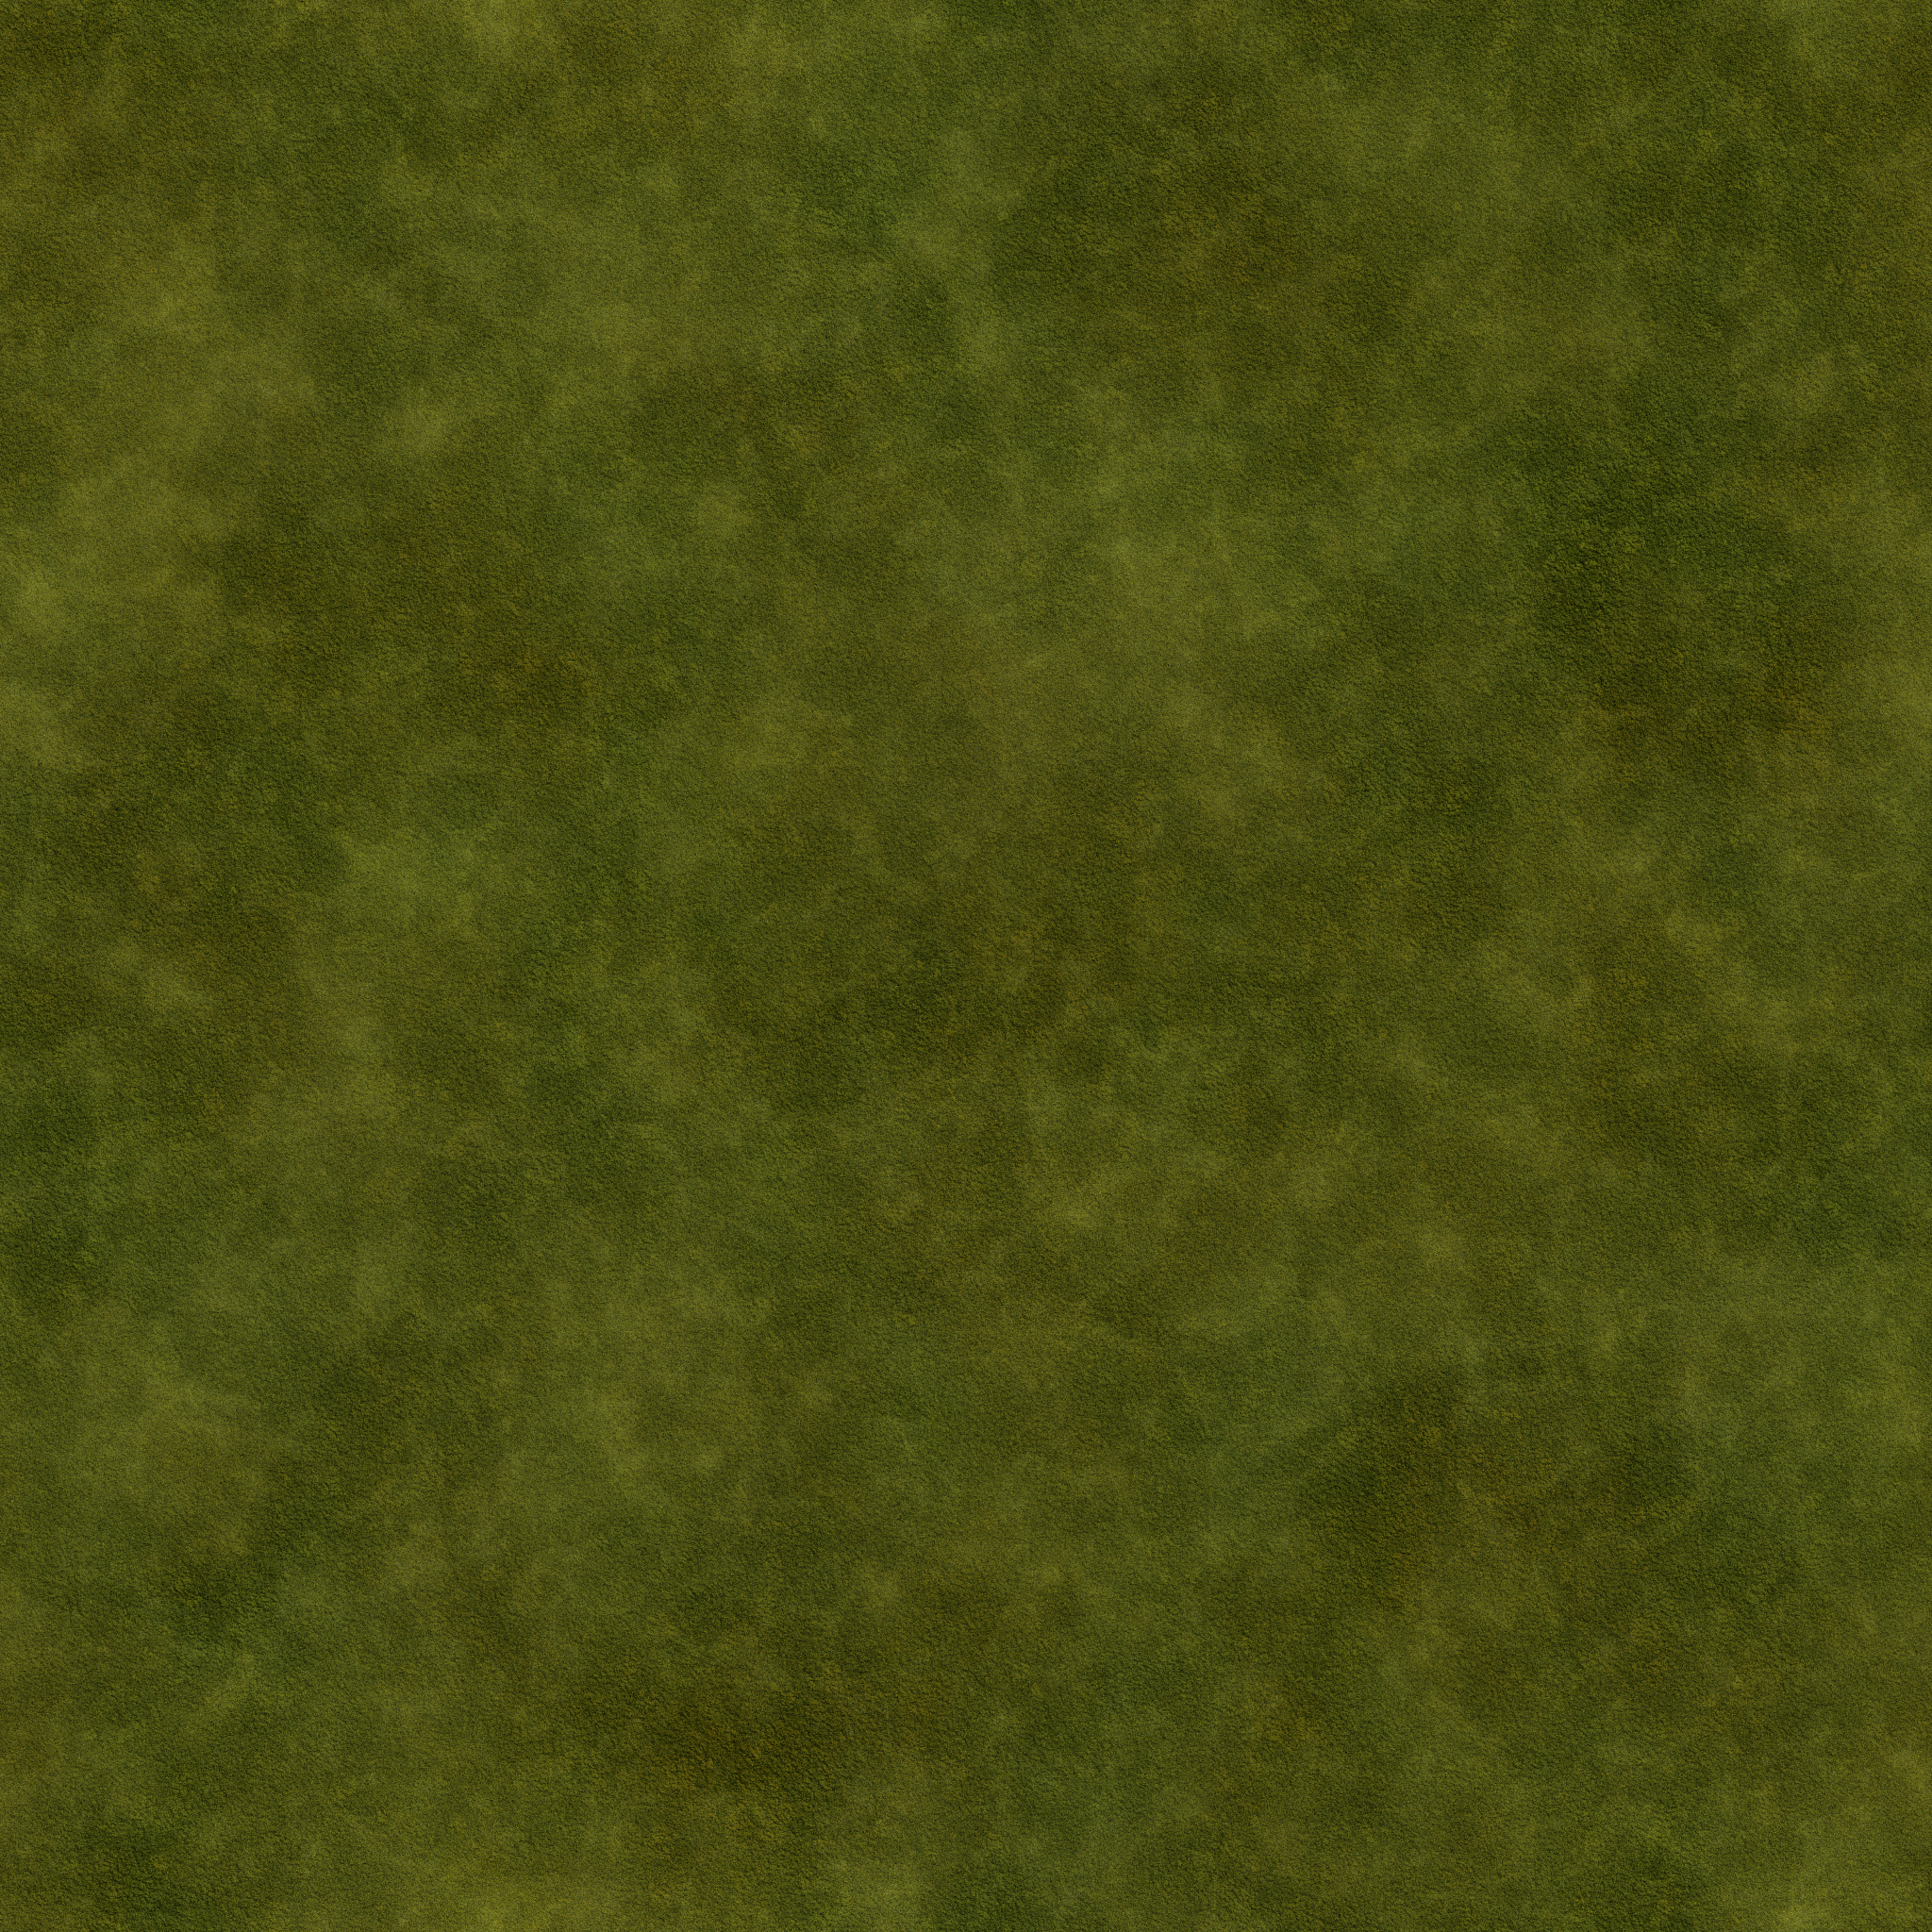
\includegraphics[width=0.9\linewidth]{images/textureGrass.jpg}
  \caption{The grass/ground texture.}
  \label{fig:textureGrass}
\end{subfigure}
\begin{subfigure}{\textwidth/3}
  \centering
  
\includegraphics[width=0.9\linewidth]{images/textureRock.jpg}
  \caption{The rock/volcano texture.}
  \label{fig:textureRock}
\end{subfigure}
\caption[Ground textures]{\textit{Textures used for the ground.}}
\label{fig:textures}
\end{figure}

The texture blending allows for the mountain to reach almost down to the ocean while still letting the fields and the highland being very grassy. The blending between rock and grass make the landscape more alive and less dull. In figure \ref{fig:textureComparison1} and \ref{fig:textureComparison2} a simple blending using linear interpolation between rock and grass is compared to our more advanced method. In our method the interpolation between the different textures vary between being squared, linear and square-root, depending on the slope and altitude.
\newpage
\begin{figure}[H]
\begin{subfigure}{0.78\textwidth}
  \centering
  \includegraphics[width=0.9\linewidth]{images/textureBlendingComparison1_simple.jpg}
  \caption{Simple linear interpolation.}
\end{subfigure}%

\begin{subfigure}{0.78\textwidth}
  \centering
  \includegraphics[width=0.9\linewidth]{images/textureBlendingComparison1_advanced.jpg}
  \caption{Advanced non-linear texture blending.}
\end{subfigure}%
\caption{A comparison between a simple interpolation of the textures (a) and our method (b). Notice the varying tone of the grass as well as the deep mountain slope to the right in (b).}
\label{fig:textureComparison1}
\end{figure}

\begin{figure}[H]
\begin{subfigure}{0.78\textwidth}
  \centering
  \includegraphics[width=0.9\linewidth]{images/textureBlendingComparison2_simple.jpg}
  \caption{Simple linear interpolation.}
\end{subfigure}

\begin{subfigure}{0.78\textwidth}
  \centering
  \includegraphics[width=0.9\linewidth]{images/textureBlendingComparison2_advanced.jpg}
  \caption{Advanced non-linear texture blending.}
\end{subfigure}
\caption{A comparison between a simple interpolation of the textures (a) and our method (b). Notice the varying tone of the grass as well as the much greener upper region to the right in (b).}
\label{fig:textureComparison2}
\end{figure}

\newpage
\subsection{Vegetation}
In order for the world to be more interesting than just an island in the middle of the sea, it needs some additional objects as well, thus plants are placed using two slightly different approaches.

First a base layer of smaller bushes and trees are placed uniformly over the landmass, with a randomized orientation and scaling. Then a few points are designated as forest centers, around these trees are placed using a Gaussian distribution, again the trees have some scale and rotation randomly selected.
\begin{figure}[H]
  \centering
  %bilden borde vara här...
  \includegraphics[width=0.9\linewidth]{images/forestfromthetop.jpg}
  \caption{Forest, viewed from the top the roughly circular shape from the gaussian used to generate it is visible}
  \label{fig:gaussainForest}
\end{figure}

Placing a tree or a bush is done by first generating a coordinate, checking it for suitability and then placing a tree if it is not unsuitable.
For example no trees can be placed in the water, or to far up on a hill.

All trees consist of two models, one trunk and one with the foilage, they aligned so that if the trunk and foilage is placed at the same coordinate, the foilage will end up in the correct place relative to the trunk.

The bushes are simple billboard models. The bushes and the trees, both textures and models, were take from TurboSquid.com.

\newpage
\begin{figure}[H]
\begin{subfigure}{0.9\textwidth}
  \centering
  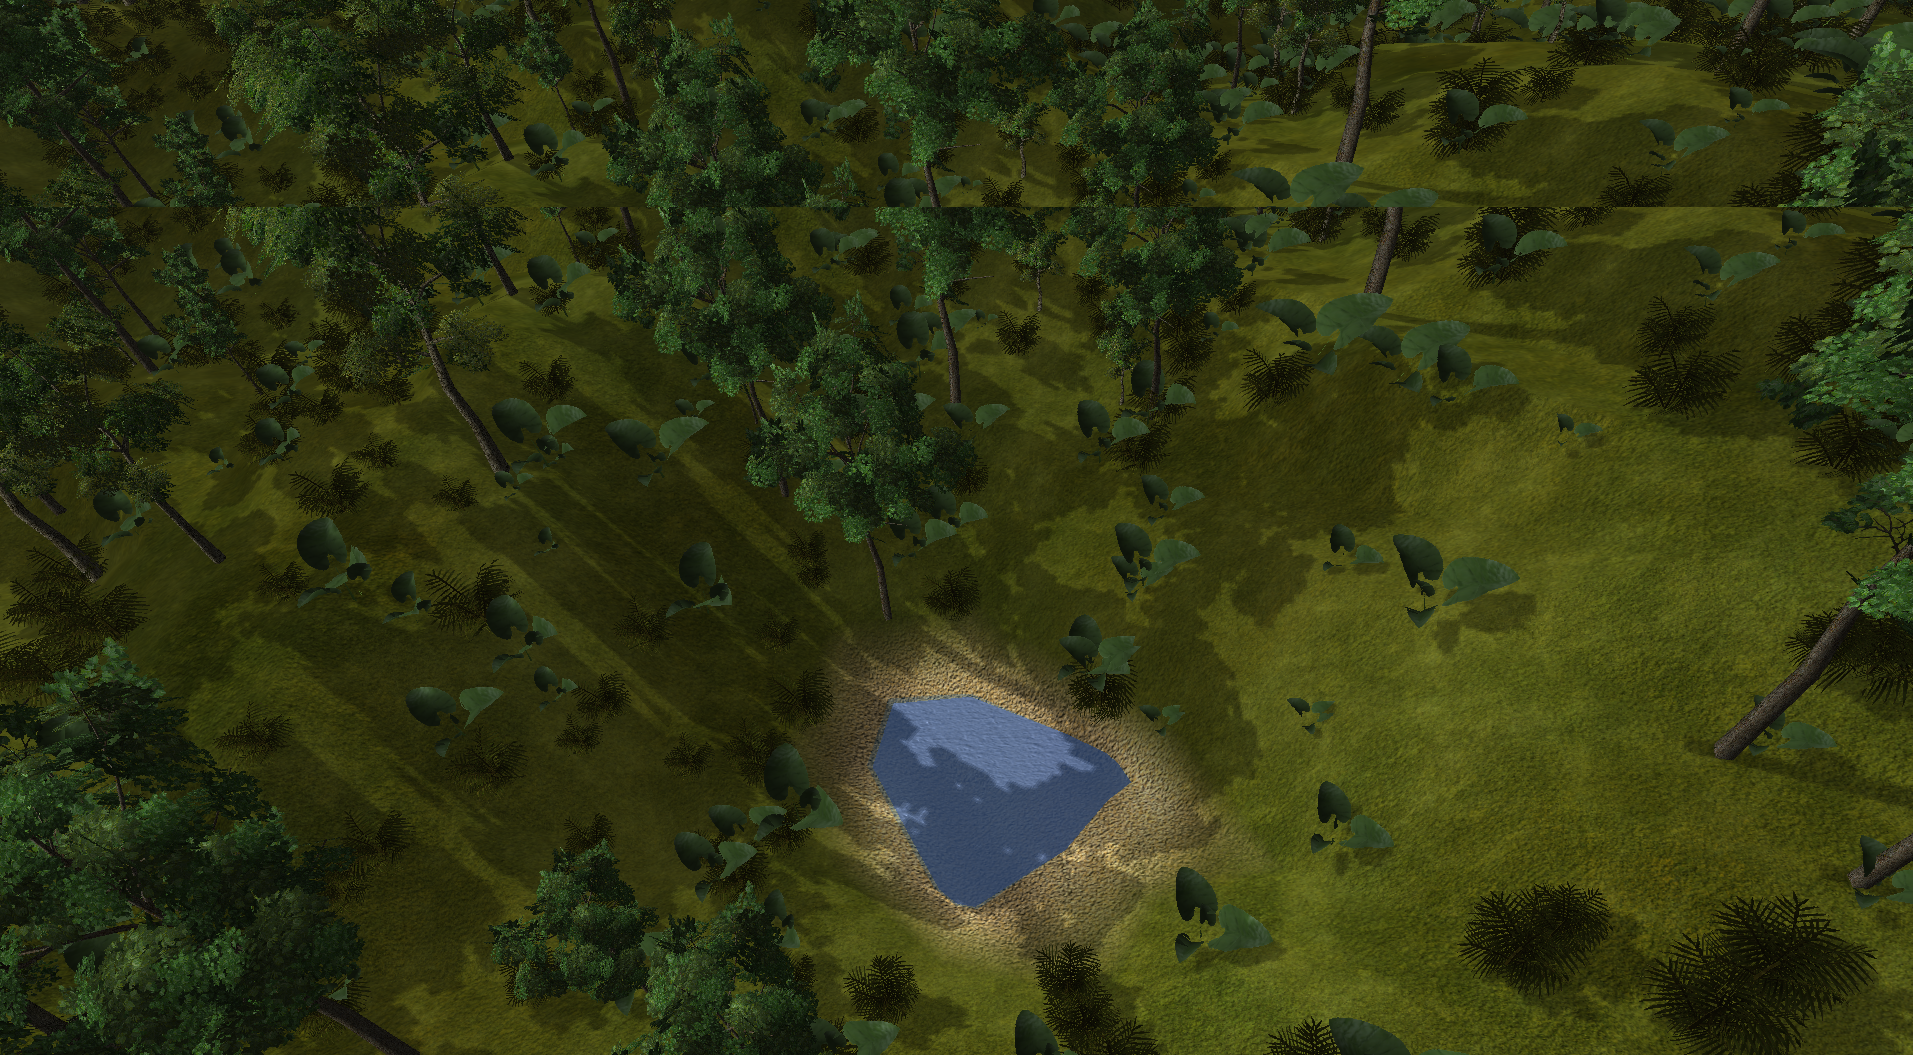
\includegraphics[width=0.9\linewidth]{images/content1.jpg}
  \caption{A small water hole in the middle of the forest at the late afternoon.}
  \label{fig:vegetation0}
\end{subfigure}%
\\
\begin{subfigure}{0.9\textwidth}
  \centering
  \includegraphics[width=0.9\linewidth]{images/vegetation1.jpg}
  \caption{The same water hole seen in (a), but perceived through the vegetation.}
  \label{fig:vegetation1}
\end{subfigure}%
\\
\begin{subfigure}{0.9\textwidth}
  \centering
  \includegraphics[width=0.9\linewidth]{images/vegetation2.jpg}
  \caption{Trees in the outskirt of a forest, portrayed against the sun.}
  \label{fig:vegetation2}
\end{subfigure}
\label{fig:vegetationViwes}
\end{figure}

\newpage
\subsection{Volcano}
The volcano generator changes the terrain on a spot to that of a volcano, such as the one seen in figure \ref{fig:volcano1}.
\begin{figure}[H]
  \centering
  \includegraphics[width=0.7\linewidth]{images/volcano.jpg}
  \caption{A volcano in full eruption.}
  \label{fig:volcano1}
\end{figure}%
\newpage
The volcano is made from one addition of a 2D-Gaussian kernel to the terrain, and of a subtraction of a smaller 2D-Gaussian kernel which creates the eruption hole. It erupts and spews out lava stones as a particle effect. The generator is currently set to generate one volcano and to place it on the highest point on the terrain.

Lava stones are made up of 5 different stone models of different sizes. They have full 3D sphere physics, including collision with each other and the terrain. Lava stones are created in the eruption hole with a randomized linear and angular momentum, forcing them to burst out of the volcano in a spraying fashion. When the lava stones enter water and sink too deep, they are re-spawned in the volcano and sent out through the hole again.

The physics can be reversed with respect to time, making the stones return to the volcano hole. When they enter the volcano they are placed where they were when they disappeared into the water last, with all the physical properties reset to how they were at that time as well. This makes lava stones come up through the water and moving in a reversed trajectory into the volcano, repeating the feat over and over, and providing a nice visual for the audience.

\begin{figure}[H]
  \centering
  \includegraphics[width=0.9\linewidth]{images/volcano3.jpg}
  \caption{A (currently) dormant volcano and its surrounding.}
  \label{fig:volcano2}
\end{figure}%

A typical volcano and its surroundings is seen in figure \ref{fig:volcano2}. In figure \ref{fig:volcanoEruptions} other views of the lava stone particle effect is shown.

\newpage
\begin{figure}[H]
\begin{subfigure}{\textwidth}
  \centering
  \includegraphics[width=0.9\linewidth]{images/Volcano1.jpg}
  \caption{A Volcano eruption seen from inside the volcano)}
  \label{fig:volcanoEruption1}
\end{subfigure}%

\begin{subfigure}{\textwidth}
  \centering
  \includegraphics[width=0.9\linewidth]{images/Volcano2.jpg}
  \caption{Volcano eruption on a small island seen from above.}
  \label{fig:volcanoEruption2}
\end{subfigure}
\caption[Noise comparison]{\textit{Volcano eruption, seen from different angles.}}
\label{fig:volcanoEruptions}
\end{figure}




\newpage

\section{Visual Effects}
Boom hacka lacka

\subsubsection{Shadows}
Shadows are one those things that can make a scene really come to life. It will help the viewer to understand the structure of the terrain and location of objects much better than with only shading. There are many techniques in which shadows can be achieved with different pros and cons. We have chosen to use \textit{Shadow Mapping} \cite{ShadowMapping} which by now is a fairly old technique, 1978, but still used in many modern computer games. Shadow mapping offers real-time shadows for arbitrary scenes in a theoretically straight forward way. 

The quality of these shadows can be increased arbitrarily, but the computational complexity grows linearly with the size of the rendered screen \cite{ShadowMapping}. Therefor one has to limit this size and go for a number of improvement techniques to make shadows shine. 

More specifically our implementation utilizes \textit{Light Space Perspective Shadow Mapping} \cite{LSPShadowMapping} which can be summarized in the following steps:

\begin{itemize}
\item Place the camera in the light source and adjust the camera frustum to cover the part of the scene that will be visible in the final render.
\item Render the scene with as simple shaders as possible and store the depth buffer. This is the shadow map.
\item Place the camera in its final-render location.
\item For each vertex:
\begin{itemize}
\item Transform into light-space coordinates.
\item Compare the distance from the light source with the corresponding value in the shadow map.
\item If the vertex is further away than the shadow map suggests, it will be shadowed. 
\end{itemize}
\end{itemize}

Once these steps got into place one could naively think that the shadows are done once and for all, but thats not the case. The result out-of-the-box looks something like figure \ref{fig:SMAcne}. The terrain is full of errors and the shadows have a pretty bad resolution. The erroneous self-shadowing on the terrain is called \textit{Shadow Acne} \cite{ImprovedShadowMapping} and is caused by precision errors in the depth test. The value in the depth map and the real depth are too close so the depth test randomly fails. This can be fixed by adding an offset to the depth value which will remove the shadow if the two depth values are too close. The improved result can be seen in figure \ref{fig:SMAcneFix}.

\begin{figure}[H]
\begin{subfigure}{.5\textwidth}
  \centering
  \includegraphics[width=0.9\linewidth]{images/SMAcne.png}
  \caption{Surface suffering from severe acne}
  \label{fig:SMAcne}
\end{subfigure}%
\begin{subfigure}{.5\textwidth}
  \centering
  \includegraphics[width=0.9\linewidth]{images/SMAcneFix.png}
  \caption{Surface healed by addition of small offset}
  \label{fig:SMAcneFix}
\end{subfigure}
\caption[Shadow mapping, acne comparison]{\textit{Comparison of shadow mapping with and without acne}}
\label{fig:AcneComparison}
\end{figure}

Care has to be taken when adding this depth offset. If the offset is to large the shadow may be disconnected from its object and cause so called \textit{Peter Paning} \cite{ImprovedShadowMapping}. A trade-off has to be made between shadow acne and peter paning. Thanks to good resolution in our depth buffers we did not need any big offset to remedy our acne problem and did therefore not suffer from any noticeable peter paning. 

The shadows now look correctly but have a very low resolution when you get close up. The edge is sharp and one can easily distinguish pixels and so pleasant may. Increasing the resolution of the shadow map depth buffer will reduce the pixel size but this will decrease the frame rate. We settled on 2048 x 2048 pixels in our buffer, figure \ref{fig:PCFLvl1}. Now my first thought was low pass filtering, and this is sort of used in the improvement technique called \textit{Percentage Closer Filtering} \cite{ShadowMapAntialiasing87}\cite{ShadowMapAntialiasing03}. By randomly sampling the surroundings of the target shadow map pixel and weighting them, in our case with a Gaussian kernel, one get a smoother shadow edge. The result is definitely an good looking improvement, figure \ref{fig:PCFLvl5}. 

\begin{figure}[H]
\begin{subfigure}{.5\textwidth}
  \centering
  \includegraphics[width=0.9\linewidth]{images/PCFLvl1.png}
  \caption{Out-of-the-box shadows}
  \label{fig:PCFLvl1}
\end{subfigure}%
\begin{subfigure}{.5\textwidth}
  \centering
  \includegraphics[width=0.9\linewidth]{images/PCFLvl5.png}
  \caption{Percentage closer filtered shadows}
  \label{fig:PCFLvl5}
\end{subfigure}
\caption[Noise comparison]{\textit{Comparison of shadow mapping with and without percentage-closer filtering}}
\label{fig:PCFComparison}
\end{figure}

One can keep tweaking these filtering methods forever but they will by themselves never become more than smoothed low-resolution shadows. To reach the next level of shadow mapping, and current industry standards, we need to look for something better. The answer seems to be \textit{Cascade Shadow Mapping} (CSM) \cite{CascadeShadowMapping}. Once I dug into this I started to see CSM everywhere. There are some characteristic transitions in the detail levels that easily can be spotted in booth BattleField 3 (2011), Counter Strike: Global Offensive (2012) and SimCity (2013), figure // TODO. My point is: this is the way to go according to the cutting-edge game industry. 

The concept is simple:

\begin{itemize}
\item Increase shadow resolution close to the camera
\item Decrease shadow resolution further away from the camera
\end{itemize}

The implementation is done by rendering several shadow maps of increasing sizes. One small map just in front of the camera and then bigger and bigger maps further away. The resolution of the maps are the same but by adjusting their sizes the pixel density is high close to the camera and lower further away from the camera. In figure \ref{fig:SMOverViewComparison} some different shadow map sizes can be seen and in figure \ref{fig:SMCloseUpComparison} the corresponding increase in quality on low-level inspection. 

\begin{figure}[H]
\begin{subfigure}{.33\textwidth}
  \centering
  \includegraphics[width=0.9\linewidth]{images/SMOverViewLvl1.png}
  \caption{Shadow mapping level 1}
  \label{fig:SMOverViewLvl1}
\end{subfigure}%
\begin{subfigure}{.33\textwidth}
  \centering
  \includegraphics[width=0.9\linewidth]{images/SMOverViewLvl2.png}
  \caption{Shadow mapping level 2}
  \label{fig:SMOverViewLvl2}
\end{subfigure}
\begin{subfigure}{.33\textwidth}
  \centering
  \includegraphics[width=0.9\linewidth]{images/SMOverViewLvl3.png}
  \caption{Shadow mapping level 3}
  \label{fig:SMOverViewLvl3}
\end{subfigure}
\caption[Noise comparison]{\textit{Overview of different shadow mapping levels}}
\label{fig:SMOverViewComparison}
\end{figure}

\begin{figure}[H]
\begin{subfigure}{.33\textwidth}
  \centering
  \includegraphics[width=0.9\linewidth]{images/SMCloseUpLvl1.png}
  \caption{Shadow mapping level 1}
  \label{fig:SMCloseUpLvl1}
\end{subfigure}%
\begin{subfigure}{.33\textwidth}
  \centering
  \includegraphics[width=0.9\linewidth]{images/SMCloseUpLvl2.png}
  \caption{Shadow mapping level 2}
  \label{fig:SMCloseUpLvl2}
\end{subfigure}
\begin{subfigure}{.33\textwidth}
  \centering
  \includegraphics[width=0.9\linewidth]{images/SMCloseUpLvl3.png}
  \caption{Shadow mapping level 3}
  \label{fig:SMCloseUpLvl3}
\end{subfigure}
\caption[Noise comparison]{\textit{Close-up of different shadow mapping levels}}
\label{fig:SMCloseUpComparison}
\end{figure}


\subsubsection{Fog}
The transition between different parts of the world can sometimes be very sharp in an unpleasant way. For instance, at the border between the sky and the ocean seen in figure \ref{fig:HorizonNoFog}. 

This can be remedied be adding some distance-fog to the ocean. If the color of the fog matches the color of the skybox at its horizon the transition will be seamless. Our skybox has been modify to fade into the color of the fog at its horizon, which can be seen in figure \ref{fig:SkyboxComparison} below. Notice that we have chosen to not let the skybox be affected by any fog. By doing so one can always see the sky when looking up, which is rather pleasant. 

\begin{figure}[H]
\begin{subfigure}{.5\textwidth}
  \centering
  \includegraphics[width=0.9\linewidth]{images/horizonNoFog.png}
  \caption{Horizon without fog}
  \label{fig:HorizonNoFog}
\end{subfigure}%
\begin{subfigure}{.5\textwidth}
  \centering
  \includegraphics[width=0.9\linewidth]{images/horizonFog.png}
  \caption{Horizon with fog}
  \label{fig:HorizonFog}
\end{subfigure}
\caption[Noise comparison]{\textit{Comparison of noise functions}}
\label{fig:HorizonFogComparison}
\end{figure}

\begin{figure}[H]
\begin{subfigure}{.5\textwidth}
  \centering
  
\includegraphics[width=0.9\linewidth]{images/skybox0.png}
  \caption{Original skybox}
  \label{fig:skybox0}
\end{subfigure}%
\begin{subfigure}{.5\textwidth}
  \centering
  
\includegraphics[width=0.9\linewidth]{images/skybox1.png}
  \caption{Skybox modified to fade into fog}
  \label{fig:skybox1}
\end{subfigure}
\caption[Noise comparison]{\textit{Comparison of skyboxes}}
\label{fig:SkyboxComparison}
\end{figure}

The distance-fog is also good for constraining the rendering size of the current scene. By adjusting the distance at which the fog appears one can adjust how much that is needed to be rendered of the scene. This enables an arbitrarily large world to be present without killing your computer since only the visible part of the world inside the fog-limit needs to be rendered. 

\subsubsection{Normal Mapping}
Normal mapping is a technique for adding fine details to an object without adding more vertices, which saves a lot of geometry computations. A normal map is generally an image where the RGB-channels represent x,y and z coordinates for a normal vector. This texture is used in the fragment shader when computing the shading for the current fragment. Before calculating the shading the normal vector is rotated to match the object on which it is to be mapped. Notice that the normal vector is not translated since we want it to remain as an normalized direction and nothing more. An example of a normal map can be seen in figure //TODO below.

// FIGURE









\newpage
\section{Artificial Intelligence}
\label{sec:AI}
Ai ai ai ai ai ai ai ai.


\newpage
\section{Conclusions}
\label{sec:conclusions}
Awesome

Possible improvements:\\
* LOD (for the vegetation)\\
* Tesselation (terrain)\\
* Living water with real waves (using tesselation)\\
* Segmentation of the world, e.g. using an occtree, to speed up the collision detection.\\
* Inhabitants of the world?



















%
% Bibliography
%

% Force a blank page so the bibliography starts on a new page.
% Comment out if not necessary
%\newpage
\thispagestyle{fancy}
\mbox{}
\begin{thebibliography}{9}
\addcontentsline{toc}{section}{References} % Add an entry for this in the table of contents

\bibitem{FracBrownMotion}
	Mandelbrot, B. \& Van Ness, J. (1968) \\ 
	``\textit{Fractional Brownian Motions, Fractional Noises and Applications}'' \\
	SIAM Review, Vol. 10, No. 4, pp. 422-437
	
\bibitem{ShadowMapping}
	Williams, L. (1978) \\ 
	``\textit{Casting Curved Shadows on Curved Surfaces}'' \\
	Computer Graphics Lab, New York Institute of Technology, Old Westbury, New York 11568 
	
\bibitem{ImprovedShadowMapping}
	Microsoft, Dev Center (2013) \\ 
	``\textit{Common Techniques to Improve Shadow Depth Maps}'' \\
	\href{http://msdn.microsoft.com/en-us/library/windows/desktop/ee416324(v=vs.85).aspx}{http://msdn.microsoft.com/en-us/library/windows/desktop/ee416324(v=vs.85).aspx}
	
\bibitem{CascadeShadowMapping}
	Microsoft, Dev Center (2013) \\ 
	``\textit{Cascaded Shadow Maps}'' \\
	\href{http://msdn.microsoft.com/en-us/library/windows/desktop/ee416307(v=vs.85).aspx}{http://msdn.microsoft.com/en-us/library/windows/desktop/ee416307(v=vs.85).aspx}
	
\bibitem{LSPShadowMapping}
	Wimmer, M., Scherzer, D. \& Purgathofer, W. (2004) \\ 
	``\textit{Light Space Perspective Shadow Maps}'' \\
	Vienna University of Technology, Austria \\

	
\bibitem{citekey}
\bibitem{citekey}

\bibitem{Gardel}
	Gardel, A., Bravo, I., Jimenez, P., Lazaro, J.L. \& Torquemada, A.\\
	``\textit{Statistical Background Models with Shadow Detection for Video Based Tracking},''\\ Intelligent Signal Processing, 2007. WISP 2007. IEEE International Symposium on?? Page: 1-6.
	
\bibitem{Zivkovic}
	Zivkovic, Z. \& Heijden, F.\\
	``\textit{Efficient Adaptive Density Estimation per Image Pixel for the Task of Background Subtraction},''\\
	Pattern recognition letters, Vol. 27, No. 7. (2006), pp. 773-780.

\bibitem{MOTA}
	Bernardin, K. \& Stiefelhagen, R (2008)\\
	``\textit{Evaluating Multiple Object Tracking Performance: The CLEAR MOT Metrics},''\\
	Interactive Systems Lab, Institut für Theoretische Informatik,\\
	Universität Karlsruhe, 76131 Karlsruhe, Germany
	
\bibitem{CAVIAR}
	``\textit{CAVIAR: Context Aware Vision using Image-based Active Recognition},''\\
	EC Funded CAVIAR project/IST 2001 37540\\
	http://homepages.inf.ed.ac.uk/rbf/CAVIAR/
	
\bibitem{StereoBM}
	Hirschmüller, H (2008)\\
	``\textit{Stereo Processing by Semiglobal Matching and Mutual Information},''\\
	IEEE Transactions on Pattern Analysis and Machine Intelligence, Volume 30(2)
	pp. 328-341.
	
\bibitem{OpenCV}
	OpenCV \textit{Open source computer vision}\\
	http://docs.opencv.org/\\
	Accessed on 2013-12-13\\
	

%\bibitem{somePaper}
%	Q. Lastname,
%	``Some article title,''
%	\emph{Some scientific journal},
%	vol.~1337, no.~1337,
%	pp.~666--1337,
%	month.~1337.

\end{thebibliography}



\end{document}
